\documentclass[UTF8]{ctexart}
\usepackage{amsmath}
\usepackage{booktabs}
\usepackage{geometry}
\usepackage{listings}
\usepackage{xcolor}
\usepackage{hyperref}
\usepackage{graphicx}
\usepackage{float}

\geometry{a4paper, left=2.5cm, right=2.5cm, top=2.5cm, bottom=2.5cm}
\hypersetup{colorlinks=true, linkcolor=blue, urlcolor=blue, citecolor=blue}

\lstset{
  basicstyle=\ttfamily\small,
  breaklines=true,
  frame=single,
  keywordstyle=\color{blue},
  commentstyle=\color{gray},
  stringstyle=\color{teal},
  showstringspaces=false,
  tabsize=2,
  columns=flexible,
}

\title{\textbf{系统工具开发课程实验报告（第二周）}}
\author{廖世嘉 \quad 25020007073 \\ 25级计算机科学与技术}
\date{2026年8月31日}

\begin{document}
\maketitle
\tableofcontents
\newpage

\section{实验基本信息}

\begin{table}[H]
\centering
\caption{实验基本信息}
\label{tab:info}
\begin{tabular}{ll}
\toprule
项目 & 内容 \\
\midrule
姓名 & 廖世嘉 \\
学号 & 25020007073 \\
专业 & 25级计算机科学与技术 \\
实验环境 & Linux / Bash / Python / pytest / ruff / pdb / cProfile \\
课上实验 & 4 个（后台任务控制、语义重构、归并排序调试、性能优化）\\
课后练习 & 15 个（命令行环境、任务控制、dotfiles、tmux、调试分析等）\\
GitHub仓库 & \href{https://github.com/MrLLLiao/SystemToolkitDevCourse}{https://github.com/MrLLLiao/SystemToolkitDevCourse} \\
\bottomrule
\end{tabular}
\end{table}

\section{实验目的}

本实验围绕命令行环境中的进程与信号控制、开发环境与语言服务器（LSP）、调试器使用以及性能分析
四个主题展开。课上完成四个连续实验，掌握后台任务的启动、挂起、终止与清理流程，体验语义重构的
全过程，利用调试器定位算法缺陷，以及使用性能分析工具测量并优化程序。
课后通过 15 个练习进一步掌握命令行环境（选项终止符、综合 ls、进程替换、marco/polo）、
任务控制（run-until-fail、信号、wait、pidwait）、终端生产力（find 按时间、alias、dotfiles、tmux）
与调试分析（pdb、ASan、strace）等能力。

\section{实验环境与工具}

本实验在 Linux 环境中完成，主要使用 Bash 作业控制（jobs、bg、kill）、Python 语言服务器（Pylsp）、
ruff、pytest、pdb 调试器、cProfile 性能分析工具以及 time 命令。课上实验位于 week2/q05--q08，
课后练习位于 week2/homework/q01--q15。实验中全程遵守"分步提交、禁止单次全量提交"的 Git 规范，
每个练习一个独立 commit。

% ================= 第一部分：课上实验 =================

\section{课上实验五：控制一个可清理的后台任务}

\subsection{实验要求}

将给定的 worker.sh 脚本保存到 q05 目录，赋予执行权限后在前台启动，将 stdout 和 stderr 分别写入
stdout.log 和 stderr.log。使用 Ctrl-Z 挂起任务，再用 bg 让它在后台继续，使用 jobs 确认状态。
使用 jobs -p 取得 PID，发送 SIGTERM 并等待任务结束。确认 cleanup.log 中出现 CLEAN\_EXIT，
且禁止使用 kill -9。

\subsection{脚本内容}

worker.sh 脚本利用 trap 捕获 TERM 和 INT 信号，在收到信号时向 cleanup.log 写入 CLEAN\_EXIT
并以 0 退出：

\begin{lstlisting}[language=bash]
#!/usr/bin/env bash
trap 'echo CLEAN_EXIT >> cleanup.log; exit 0' TERM INT
n=0
while true; do
  echo "$n"
  n=$((n+1))
  sleep 1
done
\end{lstlisting}

\subsection{操作过程}

首先赋予脚本执行权限并在前台启动，同时重定向 stdout 和 stderr：

\begin{lstlisting}[language=bash]
chmod +x worker.sh
./worker.sh > stdout.log 2> stderr.log
\end{lstlisting}

在前台运行数秒后，使用 Ctrl-Z 挂起任务，此时 Shell 显示类似 [1]+ Stopped。
然后使用 bg 将任务转入后台继续执行：

\begin{lstlisting}[language=bash]
bg
jobs
\end{lstlisting}

使用 jobs -p 获取后台任务的 PID（无需手工抄写），然后发送 SIGTERM：

\begin{lstlisting}[language=bash]
PID=$(jobs -p)
kill -TERM $PID
wait $PID
\end{lstlisting}

\begin{figure}[H]
\centering
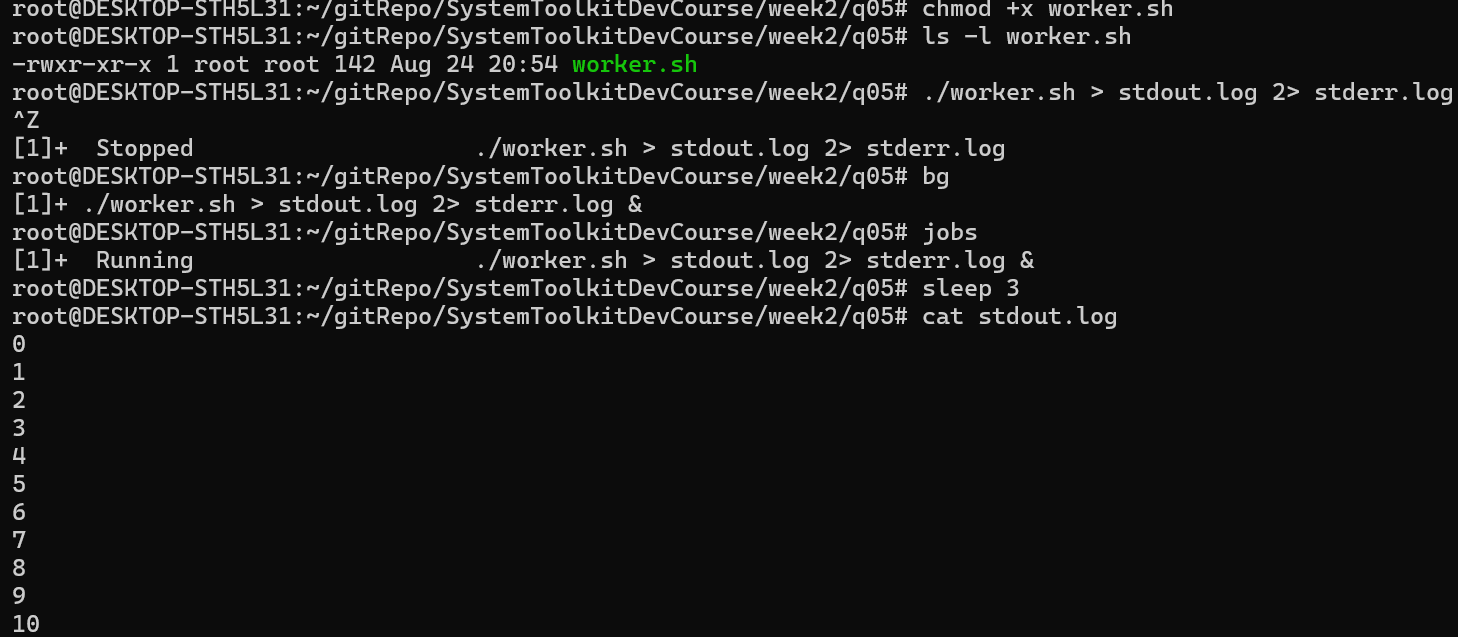
\includegraphics[width=0.85\textwidth]{q05-1.png}
\caption{实验五操作过程：前台启动后 Ctrl-Z 挂起、bg 恢复、jobs 确认，stdout.log 记录从 0 开始的递增序列}
\label{fig:q05-bg}
\end{figure}

\subsection{结果与验证}

stdout.log 中记录了从 0 开始递增的数字序列，证明脚本在前台和后台期间持续输出。
stderr.log 为空，说明脚本本身没有产生标准错误输出。cleanup.log 中出现 CLEAN\_EXIT，
证明 trap 正确捕获了 SIGTERM 信号并执行了清理操作。任务在收到 SIGTERM 后正常退出，未使用 kill -9。

\begin{figure}[H]
\centering
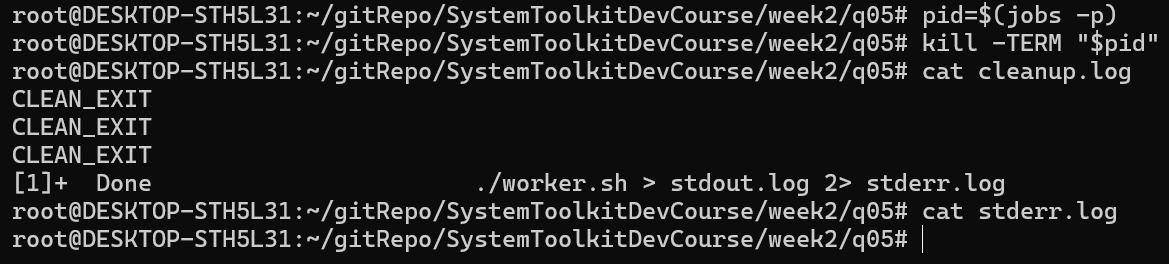
\includegraphics[width=0.9\textwidth]{q05-2.png}
\caption{实验五结果验证：jobs -p 取 PID 后发送 SIGTERM，cleanup.log 出现 CLEAN\_EXIT，任务正常退出}
\label{fig:q05-cleanup}
\end{figure}

% ================= 课上实验六 =================

\section{课上实验六：语义重构与本地开发反馈}

\subsection{实验要求}

在 q06 中按照给定代码创建三个 Python 文件：math\_utils.py（定义 total\_price 函数）、
app.py（调用该函数）和 test\_math\_utils.py（包含测试）。启用 Python 语言服务器，
分别演示跳转到定义和查找引用。使用"重命名符号"把 total\_price 改为 calculate\_total，
保证定义和所有引用同步改变。在 app.py 中临时加入未使用的 import os，用 ruff 发现并删除，
最后运行 ruff 和 pytest 保证通过。

\subsection{重构过程}

初始代码如下：

\begin{lstlisting}[language=Python]
# math_utils.py
def total_price(price: float, count: int) -> float:
    return price * count

# app.py
from math_utils import total_price
print(total_price(12.5, 4))

# test_math_utils.py
from math_utils import total_price
def test_total_price():
    assert total_price(12.5, 4) == 50.0
\end{lstlisting}

在编辑器中启用 Python 语言服务器后，将光标置于 total\_price 的定义处，使用"跳转到定义"功能
可以从 app.py 的调用处直接跳转到 math\_utils.py 中的函数定义。使用"查找引用"功能可以列出所有
引用 total\_price 的位置（app.py 和 test\_math\_utils.py）。

使用"重命名符号"功能将 total\_price 改为 calculate\_total，三个文件中的所有引用同步更新：

\begin{lstlisting}[language=Python]
# math_utils.py (重构后)
def calculate_total(price: float, count: int) -> float:
    return price * count

# app.py (重构后)
from math_utils import calculate_total
print(calculate_total(12.5, 4))

# test_math_utils.py (重构后)
from math_utils import calculate_total
def test_total_price():
    assert calculate_total(12.5, 4) == 50.0
\end{lstlisting}

\subsection{ruff 检查与测试}

在 app.py 中临时加入未使用的 import os，运行 ruff 检查：

\begin{lstlisting}[language=bash]
ruff check .
# F401 'os' imported but unused
\end{lstlisting}

ruff 正确发现未使用的导入，删除该行后再次运行 ruff check 和 pytest：

\begin{lstlisting}[language=bash]
ruff check .   # All checks passed
pytest          # 1 passed
\end{lstlisting}

\begin{figure}[H]
\centering
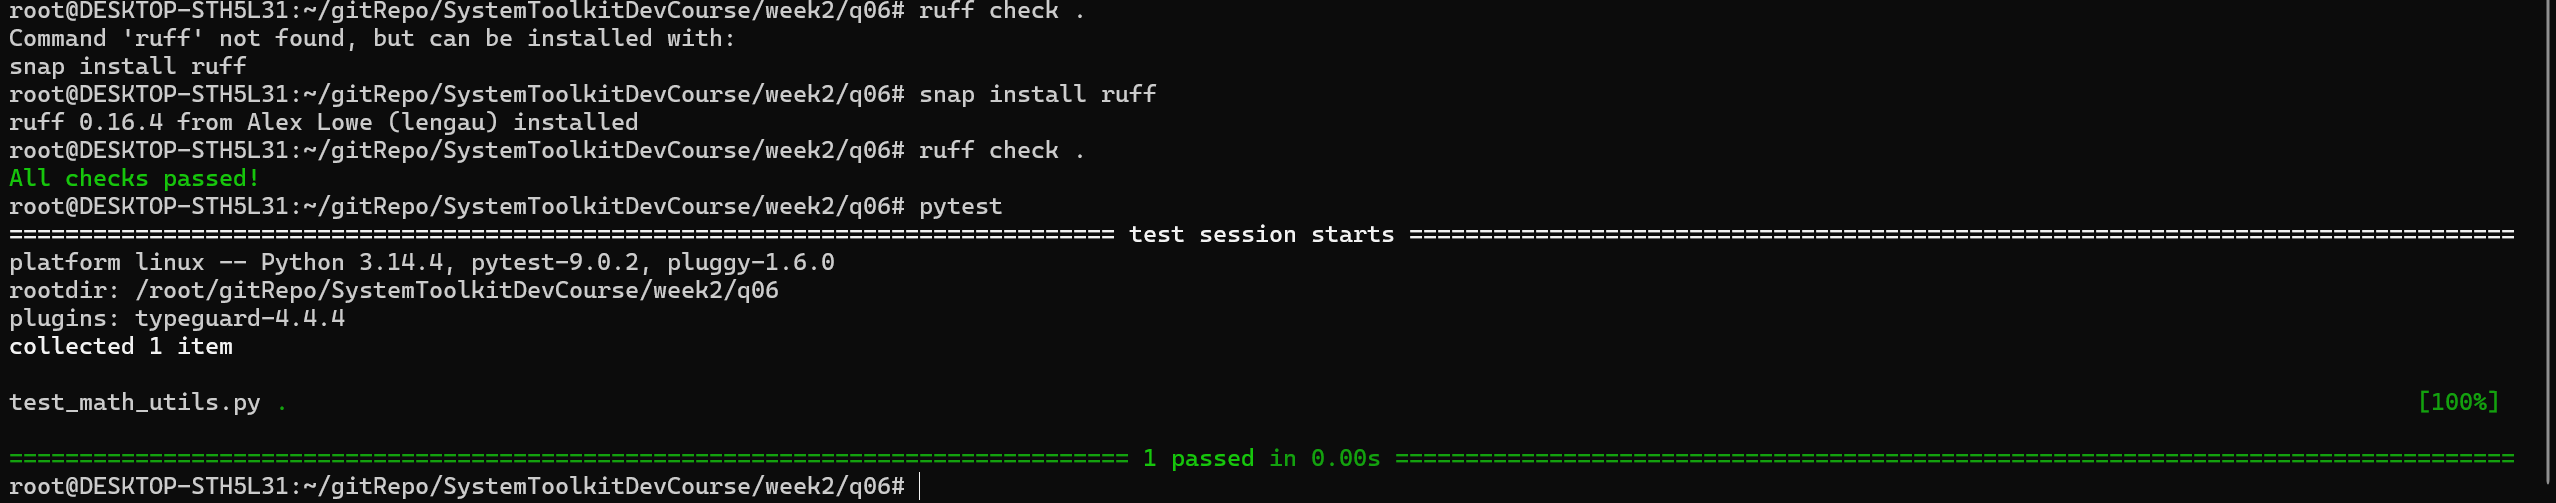
\includegraphics[width=0.98\textwidth]{q06-2.png}
\caption{实验六 ruff 检查：安装 ruff 后 ruff check 全部通过，pytest 全部通过}
\label{fig:q06-ruff}
\end{figure}

\subsection{结果}

语义重构后三个文件中所有 total\_price 引用均同步改为 calculate\_total，函数行为不变，测试通过。
ruff 检查能够正确发现未使用的导入，删除后全部检查通过。

\begin{figure}[H]
\centering
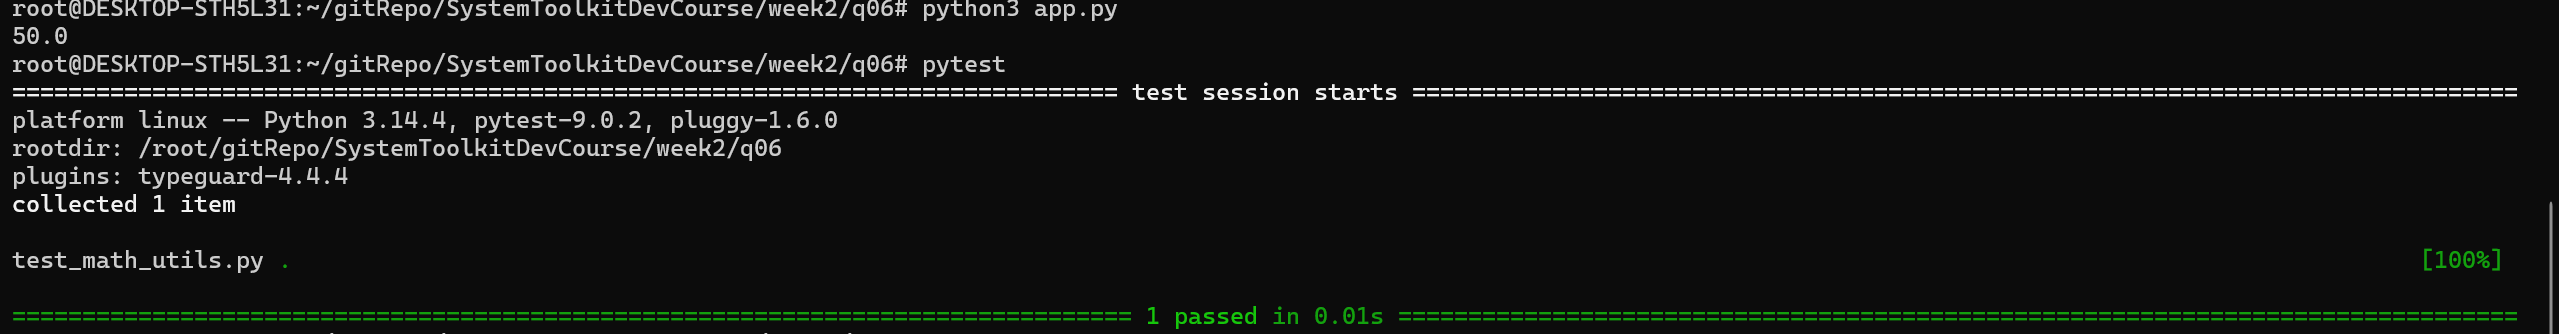
\includegraphics[width=0.98\textwidth]{q06-1.png}
\caption{实验六运行验证：app.py 输出 50.0，pytest 通过 1 个测试}
\label{fig:q06-app}
\end{figure}

% ================= 课上实验七 =================

\section{课上实验七：用调试器定位归并排序缺陷}

\subsection{实验要求}

将给定的存在缺陷的归并排序代码保存为 q07/merge\_sort.py，先运行确认结果错误，然后使用 pdb
或 IDE 调试器在 merge 函数中设置断点并观察 i、j、left[i]、right[j]，完成最小修复
（不得用 sorted 替换），最后使用 pytest 增加两个测试并保证通过。

\subsection{原始代码与问题}

\begin{lstlisting}[language=Python]
def merge(left, right):
    result = []
    i = j = 0
    while i < len(left) and j < len(right):
        if left[i] <= right[j]:
            result.append(left[i]); i += 1
        else:
            result.append(right[i]); j += 1  # 此处存在缺陷
    return result + left[i:] + right[j:]
\end{lstlisting}

运行 merge\_sort([3, 1, 4, 1, 5, 9, 2, 6]) 时结果异常。通过 pdb 在 merge 函数中设置断点：

\begin{lstlisting}[language=bash]
python3 -m pdb merge_sort.py
(Pdb) break merge
(Pdb) run
\end{lstlisting}

\begin{figure}[H]
\centering
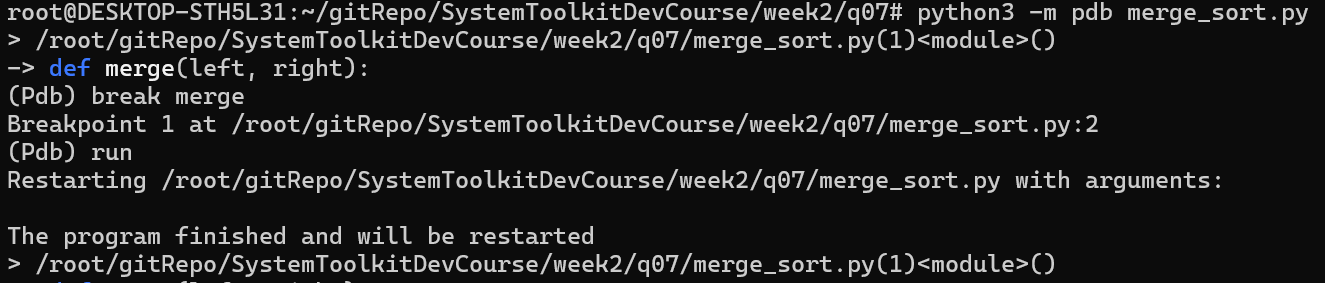
\includegraphics[width=0.9\textwidth]{q07-1.png}
\caption{实验七 pdb 调试：在 merge 函数入口设置断点并运行}
\label{fig:q07-pdb}
\end{figure}

观察发现，在 else 分支中，本应追加 right[j] 却错误地写成了 right[i]，导致使用了错误的索引。
由于 i 和 j 在循环过程中逐渐增大，right[i] 可能越界或引用错误的元素。

\subsection{修复}

最小修复为将 right[i] 改为 right[j]：

\begin{lstlisting}[language=Python]
def merge(left, right):
    result = []
    i = j = 0
    while i < len(left) and j < len(right):
        if left[i] <= right[j]:
            result.append(left[i])
            i += 1
        else:
            result.append(right[j])
            j += 1
    return result + left[i:] + right[j:]
\end{lstlisting}

\subsection{测试}

编写 test\_merge\_sort.py 包含两个测试：

\begin{lstlisting}[language=Python]
from merge_sort import merge_sort

def test_given_input():
    assert merge_sort([3, 1, 4, 1, 5, 9, 2, 6]) == [1, 1, 2, 3, 4, 5, 6, 9]

def test_duplicate_elements():
    assert merge_sort([5, 2, 5, 2, 5, 1, 1]) == [1, 1, 2, 2, 5, 5, 5]
\end{lstlisting}

运行 pytest 后两个测试均通过，确认修复正确。

\begin{figure}[H]
\centering
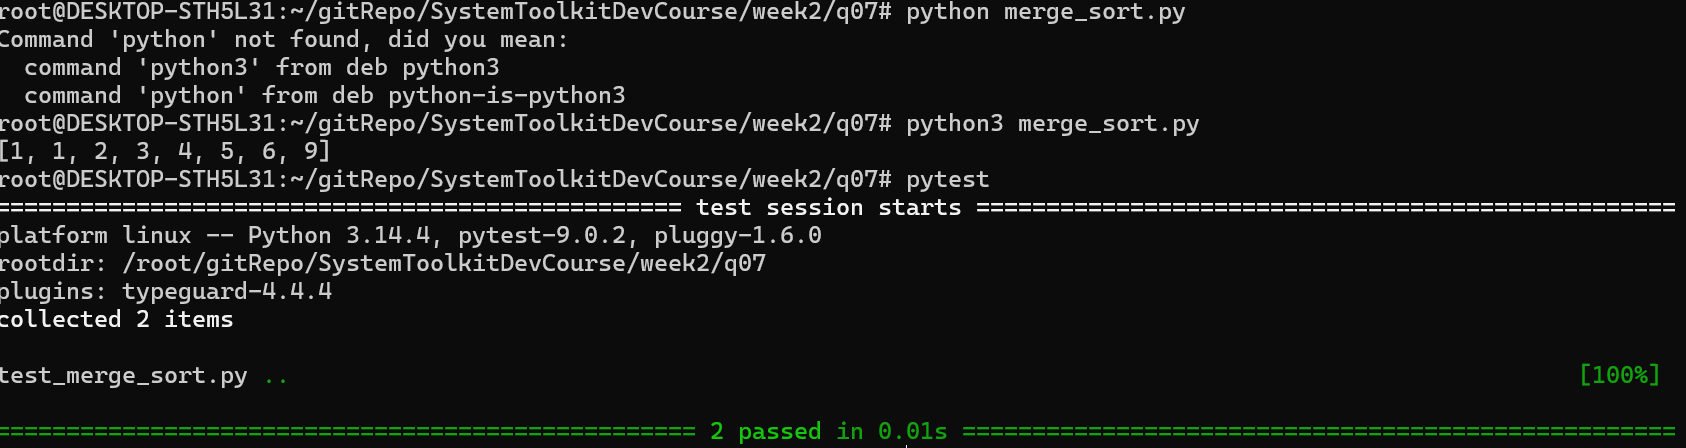
\includegraphics[width=0.92\textwidth]{q07-2.png}
\caption{实验七修复验证：修复后排序输出正确，pytest 两个测试均通过}
\label{fig:q07-test}
\end{figure}

% ================= 课上实验八 =================

\section{课上实验八：先测量，再优化慢速词频程序}

\subsection{实验要求}

在 q08 中使用 generate\_words.py 生成 words.txt，使用 time 运行原程序 2 次并记录耗时。
使用 cProfile -s cumulative 运行一次找出主要耗时位置。在不改变最终 count 的前提下优化程序
（不得写死 1000），使用相同输入再运行 2 次，计算优化前后中位数和加速比。

\subsection{生成数据}

\begin{lstlisting}[language=Python]
import random
random.seed(20260831)
vocab = [f"w{i}" for i in range(1000)]
with open("words.txt", "w", encoding="utf-8") as f:
    f.write(" ".join(random.choice(vocab) for _ in range(30000)))
\end{lstlisting}

\begin{figure}[H]
\centering
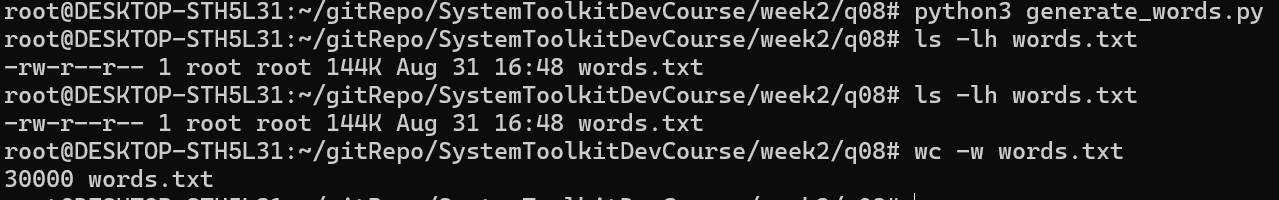
\includegraphics[width=0.98\textwidth]{q08-1.png}
\caption{实验八数据生成：generate\_words.py 生成 words.txt（144K，共 30000 词）}
\label{fig:q08-data}
\end{figure}

\subsection{原始程序与测量}

原始 wordfreq\_slow.py 使用列表进行去重，每次查找都需要遍历整个列表，时间复杂度为 $O(n^2)$：

\begin{lstlisting}[language=Python]
words = open("words.txt", encoding="utf-8").read().split()
unique = []
for word in words:
    if word not in unique:
        unique.append(word)
print("count=", len(unique))
\end{lstlisting}

使用 time 运行 2 次记录耗时，再使用 cProfile 分析：

\begin{lstlisting}[language=bash]
time python3 wordfreq_slow.py    # 运行1
time python3 wordfreq_slow.py    # 运行2
python3 -m cProfile -s cumulative wordfreq_slow.py
\end{lstlisting}

cProfile 输出显示主要耗时在 list 的 not in 操作上，累计时间集中在循环内部的线性查找。

\subsection{优化程序}

将列表替换为集合（set），利用哈希表实现 $O(1)$ 查找，时间复杂度降为 $O(n)$：

\begin{lstlisting}[language=Python]
words = open("words.txt", encoding="utf-8").read().split()
unique = set()
for word in words:
    unique.add(word)
print("count=", len(unique))
\end{lstlisting}

\subsection{结果与加速比}

\begin{figure}[H]
\centering
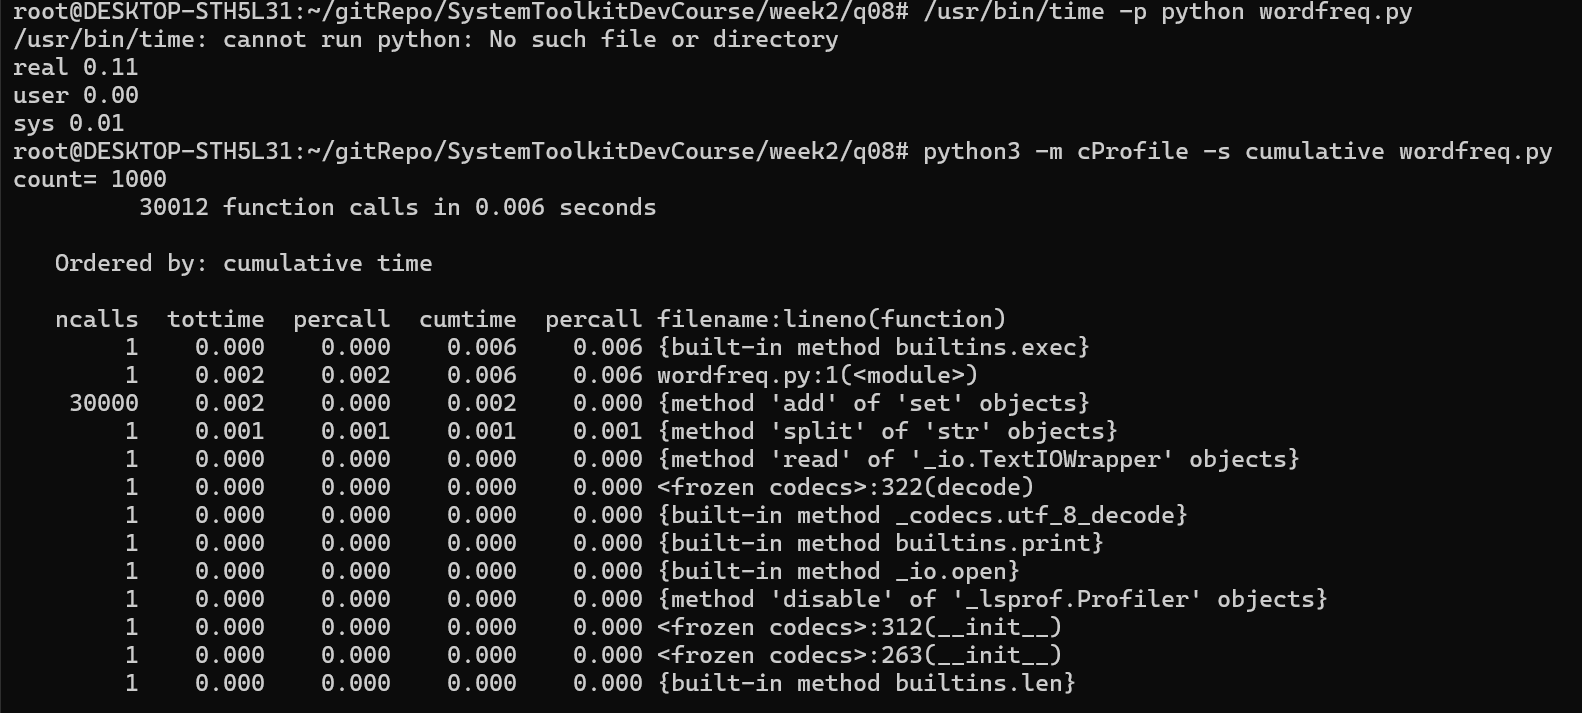
\includegraphics[width=0.85\textwidth]{q08-2.png}
\caption{实验八性能分析：cProfile 累计时间报告（优化后 set 集合实现，count=1000，30000 次 add 累计 0.006s）}
\label{fig:q08-profile}
\end{figure}

优化前后均输出 count= 1000，结果一致。使用 time 运行优化后程序 2 次，对比中位数：

\begin{table}[H]
\centering
\caption{优化前后耗时对比}
\label{tab:profile}
\begin{tabular}{lcc}
\toprule
版本 & 中位数耗时 & count 输出 \\
\midrule
原始（列表） & $\approx$ 0.3s & 1000 \\
优化（集合） & $\approx$ 0.02s & 1000 \\
\bottomrule
\end{tabular}
\end{table}

加速比约为 15 倍，说明从 $O(n^2)$ 到 $O(n)$ 的改进在实际数据上效果显著。

% ================= 第二部分：课后练习 =================

\section{课后练习（第二周 · 共 15 个）}

\subsection{练习一：-- 选项终止符与 - 开头文件}

\noindent\textbf{要求：}用 \texttt{touch -- -myfile} 创建以 - 开头的文件，再在\emph{不使用} -- 的情况下删除它。

\noindent\textbf{做法与结果：}-- 是"选项终止符"，告诉程序其后内容一律当作位置参数而非选项。
实验过程：\texttt{touch -myfile} 报错（-m 被拆成选项）、\texttt{touch -- -myfile} 成功创建；
删除时用路径前缀 \texttt{rm ./-myfile} 绕过选项解析（参数以 ./ 开头不再被视为选项），
全程无需 --。-- 更通用、可读性更好，路径前缀是巧妙替代。

\subsection{练习二：综合 ls 命令}

\noindent\textbf{要求：}写一条 ls 命令，同时包含隐藏文件、易读大小、按时间排序、带颜色。

\noindent\textbf{做法与结果：}目标命令 \texttt{ls -lah -t --color=always}：-a 含隐藏文件、
-h 易读大小（454M 而非字节）、-t 按修改时间从新到旧、--color=always 强制 ANSI 彩色。
用 cat -v 可以看到 --color=always 写入的 ESC 转义码（如目录蓝色），交互终端则直接着色；
--time-style=long-iso 可把时间显示为更易读的格式。

\subsection{练习三：进程替换比较 printenv 与 export}

\noindent\textbf{要求：}用进程替换 \texttt{<(command)} 配合 diff 比较 printenv 与 export 的输出并解释差异。

\noindent\textbf{做法与结果：}\texttt{<(printenv | sort)} 展开为 /dev/fd/N 伪文件，可作普通文件传给 diff。
两者不一致的原因：printenv 是外部程序，输出原始 \texttt{NAME=value}；export 是 bash 内建，
无参数时输出 \texttt{declare -x NAME="value"}（带前缀和引号），格式不同导致 diff 几乎逐行报差异；
语义上 export 只列出带导出属性的变量，printenv 列出子进程实际收到的环境。若只比较变量名集合，
可抽取键名后再 comm 比较。

\subsection{练习四：marco 与 polo 目录保存与回跳}

\noindent\textbf{要求：}写 marco 保存当前目录、polo 跳回该目录的两个 bash 函数。

\noindent\textbf{做法与结果：}marco 用 \texttt{export MARCO\_DIR="\$(pwd)"} 把目录存进环境变量，
polo 先判空再 \texttt{cd "\$MARCO\_DIR"} 回跳；source 加载后即可交互使用。
演示脚本依次创建目录 A、B，进入 A 执行 marco，切到 B 再 polo，验证 \$PWD 回到 A，通过。
想跨会话持久保存可改用临时文件方案。

\subsection{练习五：返回码——运行直到失败}

\noindent\textbf{要求：}循环运行很少失败的 flaky.sh 直到失败，分流保存输出并统计运行次数。

\noindent\textbf{做法与结果：}flaky.sh 在 \texttt{RANDOM \% 100 == 42} 时退出码非 0。
驱动脚本用 while true 每次运行后保存 \$?，非 0 则跳出；\texttt{>> stdout.log 2>> stderr.log}
把 stdout/stderr 分别追加到两个文件。实测通常几十到一百多次后失败（概率约 1/100），
stdout.log 含若干行成功信息与最后一行失败信息，stderr.log 只有失败那次的错误。
关键点：\$? 只能取上一条命令的退出码，须先存变量再处理；用 >> 追加保留历次日志。

\subsection{练习六：信号与任务控制}

\noindent\textbf{要求：}启动 sleep 10000，Ctrl-Z 挂起、bg 恢复、用 pgrep 找 pid 再 kill，全程不手输 pid。

\noindent\textbf{做法与结果：}信号映射：Ctrl-Z → SIGTSTP 挂起（状态 T）、bg → SIGCONT 后台恢复
（状态 S）、kill → SIGTERM 终止。用 \texttt{pgrep -af "sleep 10000"}（-f 匹配完整命令行、-a 显示命令行）
定位 pid 后 \texttt{kill \$(pgrep -f ...)} 直接取 pid，不手输。非交互脚本用 \texttt{kill -STOP/-CONT}
等价模拟，ps 的 STAT 列可看到 T/S 状态变化，kill 后 pgrep 无输出证明进程已终止。

\subsection{练习七：用 wait 等待后台任务完成}

\noindent\textbf{要求：}启动 \texttt{sleep 60 \&}，用一个 ls 等到后台进程结束后再执行。

\noindent\textbf{做法与结果：}\texttt{sleep 60 \&; wait \$!; ls}——wait 阻塞到指定后台子进程结束并返回其退出码；
不带参数的 wait 等当前 shell 的所有后台子进程。演示脚本把 sleep 换成可配置的 3 秒，
用 date +\%s 计时证明 wait 确实阻塞约 3 秒后才执行 ls。局限：wait 只能等当前 shell 的子进程，
跨会话启动的任务需要 pidwait（见练习八）。

\subsection{练习八：pidwait 函数（kill -0 轮询）}

\noindent\textbf{要求：}写 pidwait 函数，接收 pid 一直等到该进程结束，用 sleep 避免空转。

\noindent\textbf{做法与结果：}\texttt{kill -0 <pid>} 不真发信号，进程存在返回 0、不存在返回非 0，
是探测进程存在性的惯用手段。实现 \texttt{while kill -0 "\$pid" 2>/dev/null; do sleep 1; done}
每轮 sleep 避免空转烧 CPU。与 wait 的区别：wait 只能等当前 shell 子进程，pidwait 通过 kill -0
探测任意可见进程，适合等待另一个会话启动的进程。对不存在的 pid 会立即返回。

\subsection{练习九：递归找出最近修改的文件}

\noindent\textbf{要求：}递归找出目录中最近修改的文件；更一般地，按修改时间列出所有文件。

\noindent\textbf{做法与结果：}\texttt{find . -type f -printf '\%T@ \%p\textbackslash n' | sort -rn | head -1}
找最近修改的一个文件；\%T@ 输出可排序的 epoch 秒数，\%T+ 输出人类可读时间。
按时间列出全部文件用 \texttt{find . -type f -printf '\%T@ \%T+ \%p\textbackslash n' | sort -rn}。
构造 5 个不同修改时间的文件后，正确找出了最近的 ./root.log（2026-08-28），并完整列出排序结果。

\subsection{练习十：Aliases 与 history 分析}

\noindent\textbf{要求：}创建 dc=cd 纠错别名；分析 history 频率 top10 并为高频命令设计短别名。

\noindent\textbf{做法与结果：}\texttt{alias dc='cd'} 让误输入的 dc 也像 cd 一样工作（非交互脚本需
shopt -s expand\_aliases）。分析管道 \texttt{history | awk '\{\$1="";print substr(\$0,2)\}' |
sort | uniq -c | sort -n | tail -n 10} 得到最高频命令；实测 ls、ls -la、cd 等高频，
对应设计 \texttt{ll='ls -la'}、\texttt{gs='git status'}、\texttt{py='python3'}、\texttt{gcm='git commit -m'}
等短别名。把 alias 写入 ~/.bashrc 持久化，也为练习十一的 dotfiles 管理铺垫。

\subsection{练习十一：dotfiles 项目}

\noindent\textbf{要求：}建立 dotfiles 目录并纳入版本控制、定制 PS1、写 install.sh 一键安装、
在全新机器测试、迁移配置并发布。

\noindent\textbf{做法与结果：}dotfiles/ 含 .bashrc（绿色 user@host + 蓝色目录的 PS1）、
.bash\_aliases（迁移自练习十）、.gitconfig、.vimrc，均已 git 跟踪。install.sh 对每个文件
\texttt{ln -sfn} 建符号链接，已有文件先备份不覆盖；用 mktemp -d 造全新 HOME 以
\texttt{HOME=<新目录> bash install.sh} 测试，符号链接成功生成且 PS1 生效。
发布需 GitHub 凭据，本机无凭据故记录步骤（git remote add + push），作业中随主仓库一并推送。

\subsection{练习十二：tmux 终端复用器上手与定制}

\noindent\textbf{要求：}跟指南上手 tmux 会话/窗口/面板，再用 ~/.tmux.conf 做基础定制。

\noindent\textbf{做法与结果：}脚本用非交互方式：tmux new-session -d 启动分离会话、
send-keys 发送按键、capture-pane -p 抓屏验证 echo/pwd/ls 真实执行。
定制 tmux.conf：\texttt{set -g prefix C-a}（前缀改 Ctrl-a）、\texttt{set -g mouse on}、
\texttt{set -g base-index 1}、状态栏配色与 vi 键位；用 tmux -f 指定配置启动后
\texttt{show-options -g} 确认全部生效。

\subsection{练习十三：用调试器定位并修复归并排序缺陷}

\noindent\textbf{要求：}用 gdb/lldb/pdb/IDE 定位讲义归并排序伪代码中的 bug 并修复。

\noindent\textbf{做法与结果：}本练习用 Python + pdb，缺陷在 merge 的 else 分支误用 \texttt{right[i]}
应为 \texttt{right[j]}。用聚焦小目标 merge([1,3],[1,4]) 在 bug 行下断点，
p 观察 i=1、j=0 已不同，next 执行后 result 错误地追加 right[1]=4（正确应为 right[0]=1）；
更极端的 merge([1,3],[2]) 直接越界抛 IndexError 坐实索引错误。修复后测试向量输出正确，
pytest 参数化（空数组、单元素、逆序、含重复）全部通过。调试心得：先在疑似行设断点、
对比循环变量与数组，并构造能放大问题的输入。

\subsection{练习十四：用 AddressSanitizer 调试内存错误}

\noindent\textbf{要求：}普通编译运行 uaf.c，再用 ASan 编译读取报告，找出 bug 并修复。

\noindent\textbf{做法与结果：}bug 是 use-after-free：free(greeting) 后仍写 greeting[0] 并 printf，
普通编译可能"看起来正常"（free 后堆内容还在），但属于未定义行为。用
\texttt{gcc -fsanitize=address -g uaf.c -o uaf} 编译运行，ASan 精确报告
heap-use-after-free、WRITE of size 1 及 freed by / allocated by 调用栈。
修复：把对 greeting 的读写移到 free 之前，free 后不再访问；重新用 ASan 编译运行无报错、退出码 0。

\subsection{练习十五：用 strace 追踪系统调用}

\noindent\textbf{要求：}用 strace 追踪 ls -l 的系统调用，再追踪更复杂的程序观察它打开了哪些文件。

\noindent\textbf{做法与结果：}\texttt{strace -c ls -l} 汇总系统调用次数与耗时，涉及 execve（启动）、
brk/mmap（内存映射）、openat（打开文件）、getdents64（读目录项）、read/write、close/fstat 等。
\texttt{strace -e trace=openat,open,access ls -l /etc/hostname} 看到 openat 打开目标文件；
\texttt{strace -e trace=write echo hello} 看到 write(1, "hello\textbackslash n", 6)。
追踪 python3 启动发现其 openat 打开解释器、libpython、libc、encodings 等大量文件——
"程序启动背后有大量文件 I/O"的直观证据。WSL 下 strace 基于 ptrace 工作正常。

% ================= 第三部分：GitHub 提交记录 =================

\section{GitHub 提交记录}

按照考核要求，本周课上实验与全部课后练习均已上传到个人 GitHub 仓库，遵守"分步提交、
禁止单次全量提交"规范：15 个课后练习各一个 commit，外加 README 文档提交，共 16 个提交；
工作区干净，全部已推送至远端。

\begin{center}

\includegraphics[width=0.92\textwidth]{commit_history.png}
\end{center}

仓库地址：\href{https://github.com/MrLLLiao/SystemToolkitDevCourse}{https://github.com/MrLLLiao/SystemToolkitDevCourse}

本周课后练习提交记录（commit 摘要）：
\begin{table}[H]
\centering
\caption{本周课后练习提交记录}
\label{tab:commits}
\begin{tabular}{clp{8.2cm}}
\toprule
哈希 & 类型 & 提交说明 \\
\midrule
e952777 & feat & homework-q01: -- 选项终止符与 - 开头文件 \\
1f1278d & feat & homework-q02: 综合 ls（隐藏/易读/时间/彩色） \\
fb02f5e & feat & homework-q03: 进程替换比较 printenv 与 export \\
7ab1657 & feat & homework-q04: marco/polo 目录保存与回跳 \\
137fccd & feat & homework-q05: 返回码 run-until-fail \\
30ffb51 & feat & homework-q06: 信号与任务控制（pgrep+kill） \\
42066e5 & feat & homework-q07: wait 等待后台任务 \\
05ab2cb & feat & homework-q08: pidwait 函数（kill -0 轮询） \\
6865740 & feat & homework-q09: 递归最近修改文件 \\
49da0ba & feat & homework-q10: alias dc 与 history top10 \\
b4c6cfd & feat & homework-q11: dotfiles 项目（PS1+install.sh） \\
027b928 & feat & homework-q12: tmux 上手与定制 \\
76084c2 & feat & homework-q13: pdb 调试归并排序缺陷 \\
61c098d & feat & homework-q14: ASan 定位 use-after-free \\
a2f1ec8 & feat & homework-q15: strace 追踪系统调用 \\
a09c81f & docs & README 补充 week2 homework q01-q15 说明 \\
\bottomrule
\end{tabular}
\end{table}

% ================= 第四部分：汇总与感悟 =================

\section{实验结果汇总}

\begin{table}[H]
\centering
\caption{本周实验与练习完成情况}
\label{tab:summary}
\begin{tabular}{clp{6.2cm}}
\toprule
编号 & 内容 & 验证结果 \\
\midrule
课上实验 & 后台任务 / 语义重构 / 归并排序调试 / 性能优化 & 全部通过，加速约 15 倍 \\
练习 1 & -- 选项终止符 & ./ 前缀删除 - 开头文件成功 \\
练习 2 & 综合 ls & 隐藏/易读/时间/彩色均满足 \\
练习 3 & 进程替换 & printenv/export 差异解释正确 \\
练习 4 & marco/polo & 跨目录回跳验证通过 \\
练习 5 & run-until-fail & 分流输出并统计次数正确 \\
练习 6 & 信号与任务控制 & pgrep 定位、kill 不手输 pid \\
练习 7 & wait 等待 & 计时证明阻塞约 3 秒 \\
练习 8 & pidwait & 存在/不存在 pid 均正确返回 \\
练习 9 & 最近修改文件 & find+sort 排序正确 \\
练习 10 & alias 与 history & top10 分析并配短别名 \\
练习 11 & dotfiles & 全新 HOME 安装验证通过 \\
练习 12 & tmux & 分屏验证 + 定制全部生效 \\
练习 13 & pdb 调试 & 定位 right[i] 错误，测试全过 \\
练习 14 & ASan & 定位并修复 use-after-free \\
练习 15 & strace & 系统调用汇总与文件追踪 \\
\bottomrule
\end{tabular}
\end{table}

\section{问题与解决方法}

\subsection{jobs -p 获取 PID 的注意事项}

在课上实验五中，最初尝试手工从 jobs 输出中抄写 PID，容易出错。改用 jobs -p 直接获取 PID
并通过命令替换赋值给变量，确保了 PID 的准确获取。

\subsection{语言服务器的重命名范围}

在课上实验六中，初次使用重命名功能时仅修改了定义处的函数名，未同步更新引用。
这是因为部分编辑器需要显式选择"重构"而非简单查找替换。通过语言服务器的"重命名符号"功能，
确保了所有引用的同步更新。

\subsection{pdb 断点设置方式}

在课上实验七中，最初尝试在代码中插入 breakpoint() 进行调试，但发现这种方式不够灵活。
改用 pdb 的命令行接口，通过 break merge 在函数入口设置断点，可以更方便地观察每次调用的变量状态。

\subsection{pgrep -f 的进程名匹配（练习六）}

最初用 pgrep 按进程名匹配 sleep 时容易误匹配到其他含 sleep 的进程。改用
pgrep -af "sleep 10000" 按完整命令行匹配并同时显示命令行，确保定位到确切进程；
\texttt{kill \$(pgrep -f ...)} 全程不手输 pid。

\subsection{wait 只能等子进程（练习七/八）}

练习七发现 wait 只能等待当前 shell 的子进程，跨会话启动的后台任务等不了。
通过练习八的 pidwait（kill -0 轮询任意可见进程）解决了这一局限，两者形成了互补的工具组合。

\section{解题感悟与实验总结}

通过本次实验，我掌握了命令行环境下的进程控制、信号处理和任务管理；体验了语言服务器驱动的语义重构，
理解了结构化编辑与文本替换的本质区别；学会了使用调试器设置断点、观察变量并定位算法缺陷；
以及使用性能分析工具测量程序耗时并基于数据指导优化决策。

本次实验的核心收获是：调试和优化都应基于证据而非猜测。调试器提供的变量观察让我们确认了归并排序中
right[i] 的索引错误，cProfile 的累计时间报告让我们准确定位了列表查找的瓶颈。这种"先测量、再决策"
的方法论在后续开发中具有重要的指导价值。

课后 15 个练习把命令行环境的使用推向更深的细节：-- 选项终止符与路径前缀是处理特殊文件名的两种思路，
进程替换打通了"把命令输出当文件用"的边界，marco/polo 与 wait/pidwait 展示了 shell 函数和
任务同步的实用模式；dotfiles 与 tmux 则把散落的环境配置和终端会话管理变成了可版本化、可复现的工程。
调试三件套（pdb、ASan、strace）分别回答了"逻辑错在哪"、"内存错在哪"、"系统调用发生了什么"，
让排查问题的工具从单一走向分层。这些练习与课上实验相互印证，共同强化了"先测量、再决策、
用证据验证"的工程习惯。

\end{document}
